\section{Simulation Results}
\label{sec:results}
This section discusses the results of the numerical experiments
evaluating the performance of the DZ MVDR ABF. The experiments are
conducted for two cases: (1) stationary interferers and (2) a moving
interferer. In the stationary interferer cases, the DZ MVDR ABF is
compared with the SMI MVDR and the DL MVDR ABFs. In the moving
interferer case, the DZ MVDR ABF is compared with the CMT MVDR ABF.
In the experiments, all ABFs are implemented using an $N = 31$ element
standard ULA and steered to broadside ($\ulook = 0$). The experiments
assume a passive sonar application where ABFs commonly operate with
barely sufficient snapshots $L = N + 1$ and even $L = 2N$ snapshots
is a relatively snapshot rich case
\cite{cox2002adaptive,baggeroer1999passive}. For all experiments, the
simulated snapshots consists of interferers and unit power white
background noise. No source signal is present in the simulated
snapshot data. All results discussed below are obtained from 3000
trials Monte Carlo experiment.

\subsection{Stationary interferer case}
\label{sec:stat-interf}
Stationary interferers maintain a fixed direction during the snapshot
averaging interval. Two scenarios with stationary interferers are
considered for evaluation of the ABFs. The first scenario has a single
narrowband interferer present at direction $\uinter = 3/N$ with $40$
dB of INR. The second scenario has four discrete narrowband
interferers at directions $\uinter = \{-7/N, ~-3/N, ~3/N, ~7/N \}$
with $\{30, ~20, ~20, ~30 \}$ dB of INR respectively.

\figurename{}~\ref{fig:pout-ecdf} shows the empirical cumulative
distribution function (ECDF) of the output power from the DZ MVDR ABF
compared with the SMI MVDR, and the DL MVDR ABFs. The left panels show
the ECDF graphs for the snapshot limited case ($L = 32$) and the right
panels show the ECDF graphs for the snapshot sufficient case
($L = 62$). The dotted vertical line in each panel denotes the
ensemble output power ($P_{\rm ens}$) produced by the MVDR beamformer
implemented using the knowledge of the ECM. The ensemble output power
is the ideally possible minimum output power for the experimental
scenario. The output power level corresponding to the ECDF value of
$0.5$ denotes the median output power. The closer the median is to the
dotted vertical line, higher the probability of the ABFs to produce
output power comparable to the ensemble output power. The DL factor
for the DL MVDR ABF is set to match the average WNG between the DL
MVDR ABF and the DZ MVDR ABF in each case.

In all four cases in \figurename{}~\ref{fig:pout-ecdf} the DZ MVDR ABF
exhibits higher probability of producing lower output power compared
to the SMI MVDR and the DL MVDR ABF, over the observed output power
range. When snapshot limited ($L = 32$), the DZ MVDR median output
power is less than the SMI MVDR ABF median output power by a factor of
ten. When snapshot sufficient ($L = 62$) the DZ MVDR median output
power is less than the SMI MVDR ABF median output power approximately
by a factor of $1.5$. The DZ MVDR ABF exhibits the greatest
improvement over the SMI MVDR ABF in the snapshot limited
cases. Moreover, the DZ MVDR ABF achieves consistently lower median
output power independent of the snapshots for both single and multiple
interferer scenarios. In contrast, the SMI MVDR ABF's output is
sensitive to the number of snapshots available.

For all interferer scenarios and snapshot conditions, the ECDF of the
DZ MVDR ABF is comparable with the DL MVDR ABF which has the same
average WNG. Examining the snapshot limited ($L = 32$) case for both
single and multiple interferer scenario the DZ MVDR ABF has lower
median output power than the DL MVDR ABF. The lower output power
indicates that the DZ MVDR ABF suppresses the interferer and noise
better than the DL MVDR ABF. In the snapshot sufficient ($L = 62$)
case for both single and multiple interferer scenario, the DZ MVDR and
the DL MVDR ABF have essentially equal median output power. However
the DL MVDR ABF requires a prior choice of the DL factor whereas the
DZ MVDR ABF achieves same performance without the need to choose a
design parameter.

\begin{figure*}[!hp]
  \centering
  \subfloat[Single interferer, L = 32]  {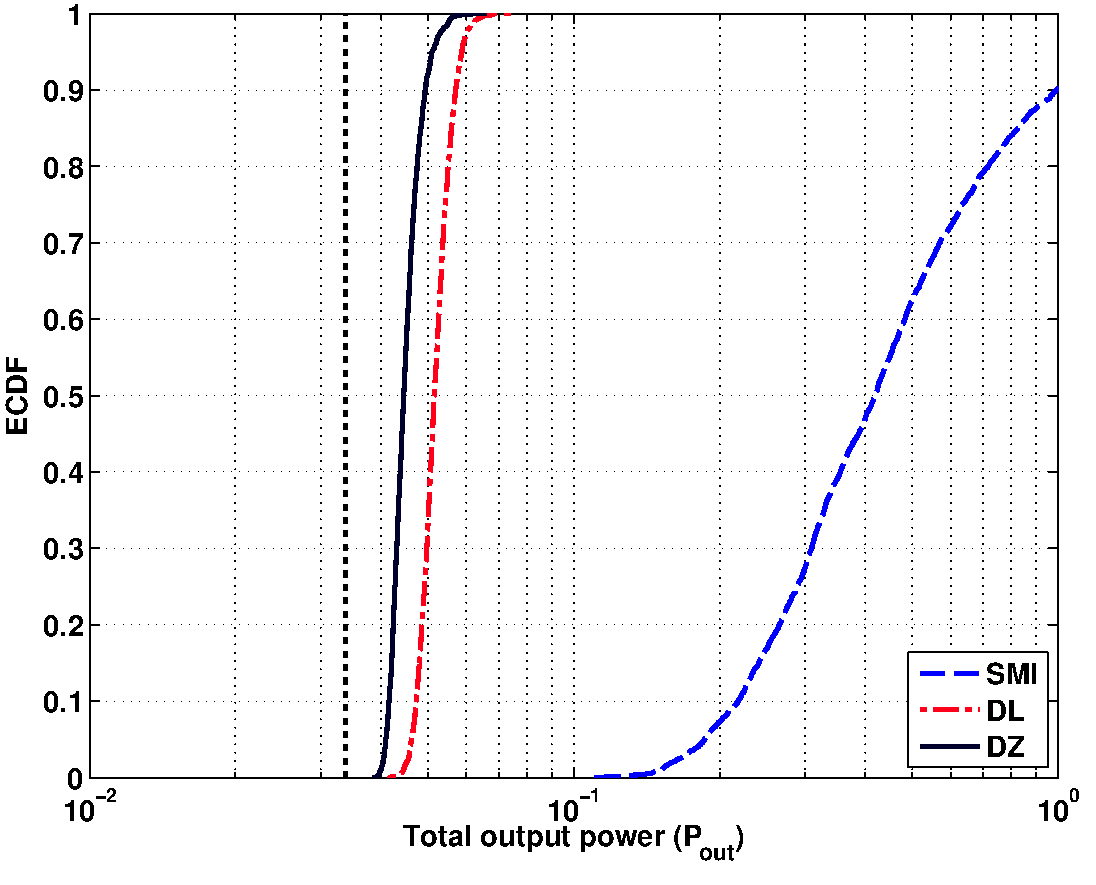
\includegraphics[width=3in]{total_pout_ecdf_single_interf_N31_L32_INR40.pdf}%
    \label{fig:pout-s-L32}}
\subfloat[Single interferer, L = 62]
{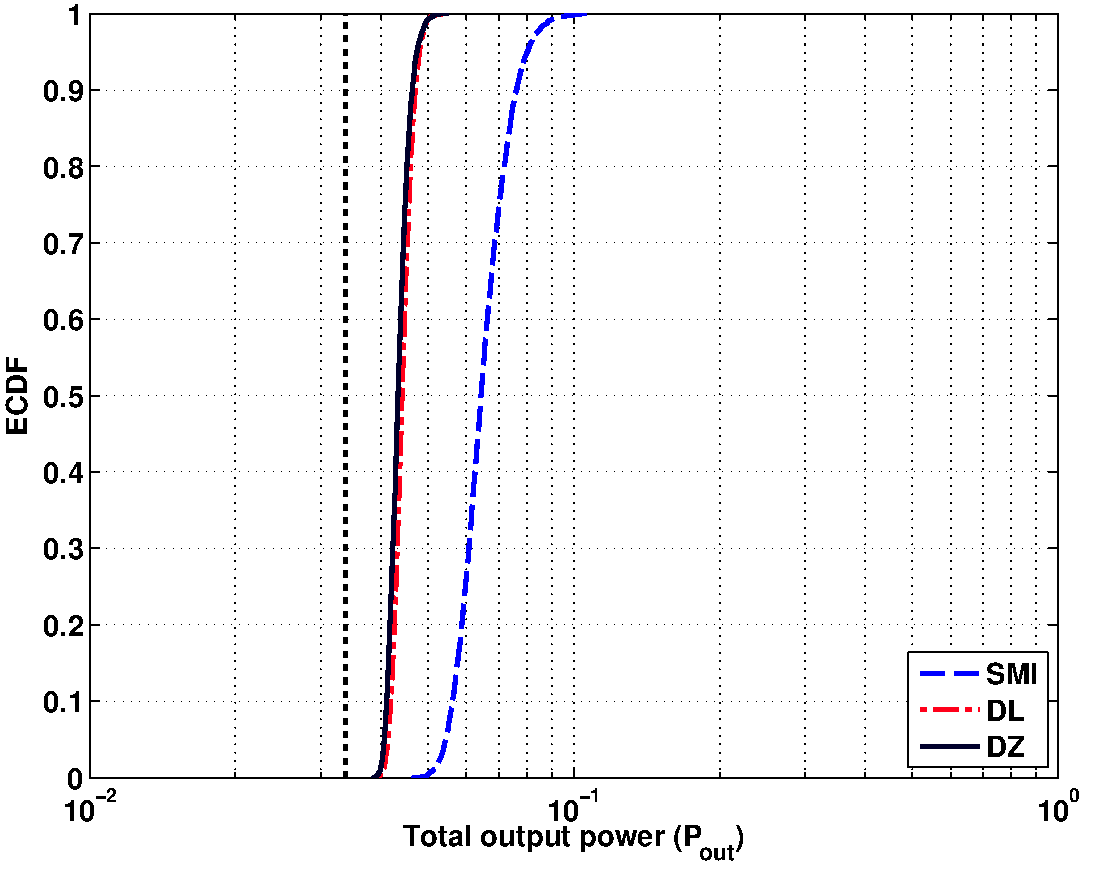
\includegraphics[width=3in]{total_pout_ecdf_single_interf_N31_L62_INR40.pdf}%
    \label{fig:pout-s-L62}}

  \subfloat[Multiple interferers, L = 32]
  {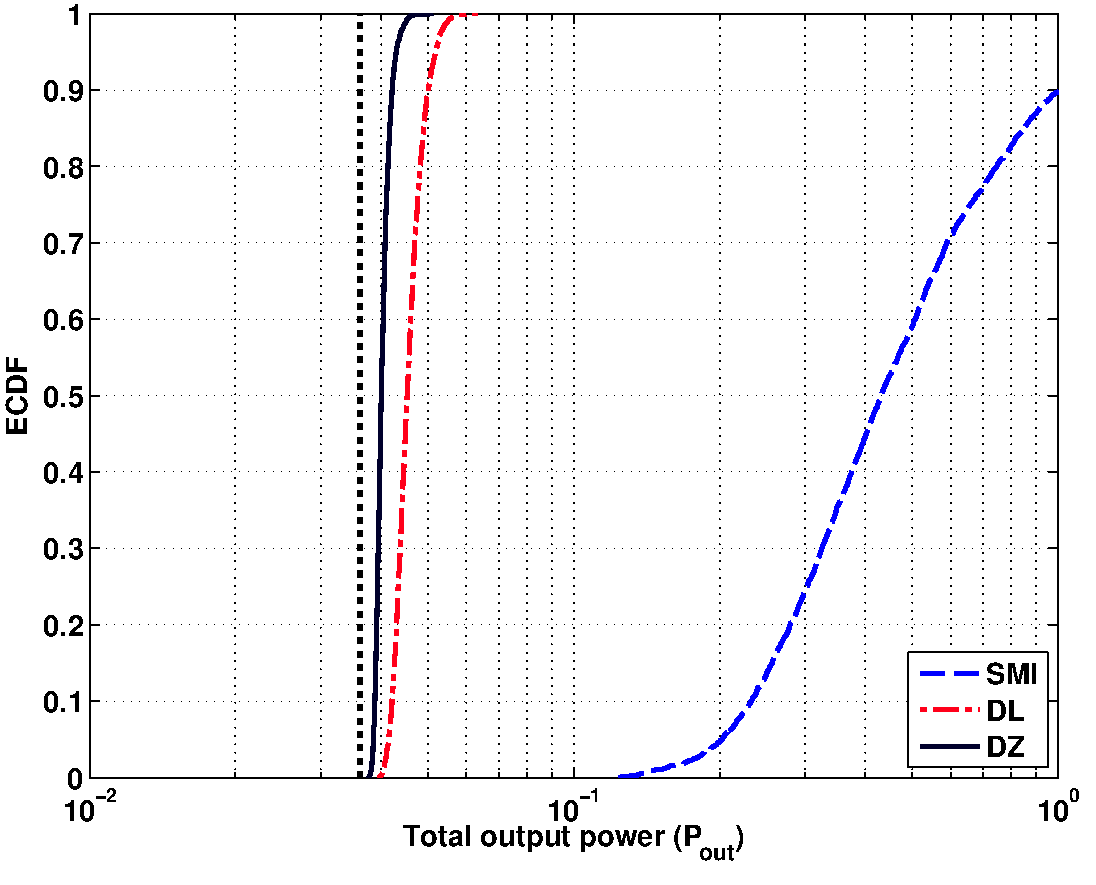
\includegraphics[width=3in]{total_pout_ecdf_multi_interf_N31_L32.pdf}%
    \label{fig:pout-m-L32}}
  \subfloat[Multiple interferers, L = 62]
  {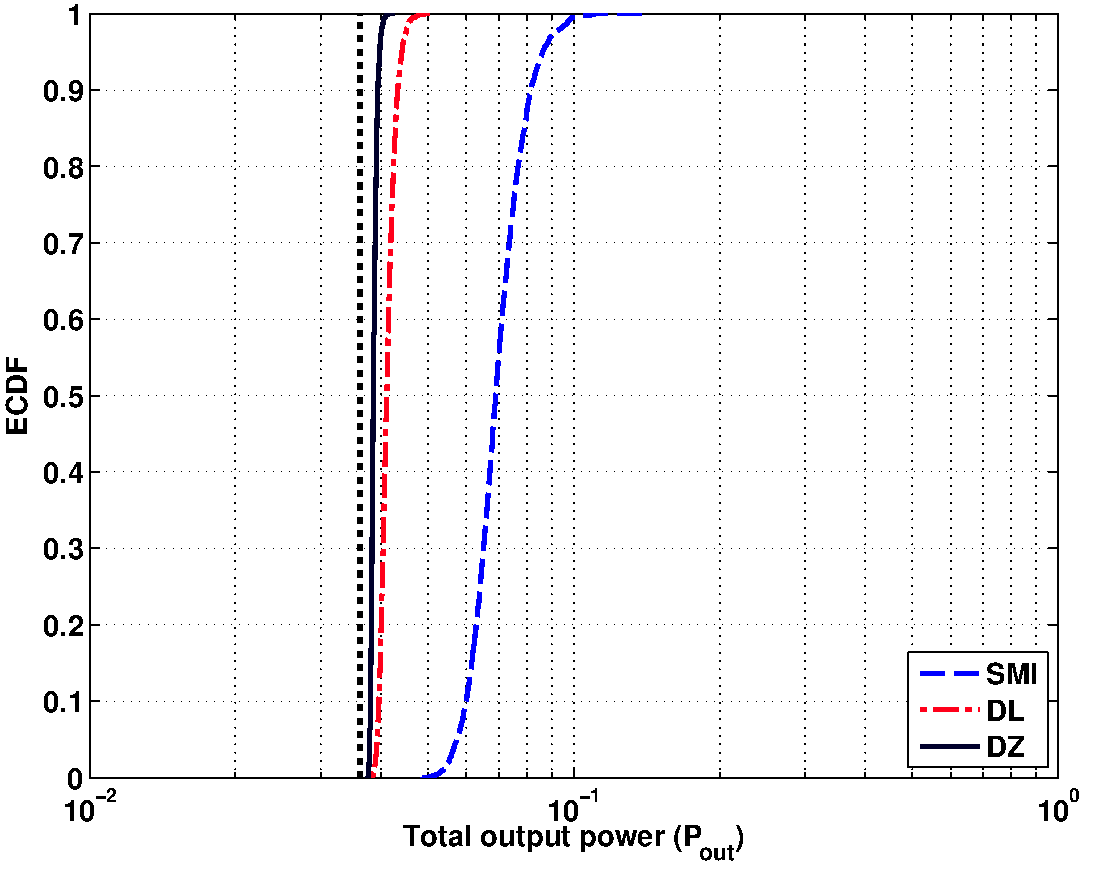
\includegraphics[width=3in]{total_pout_ecdf_multi_interf_N31_L62.pdf}%
    \label{fig:pout-m-L62}}
  \caption[Output power ECDF for the SMI MVDR, DL MVDR and the DZ MVDR
    ABFs using an $N = 31$ element ULA]{Output power ECDF for the SMI MVDR, DL MVDR and the DZ MVDR
    ABFs using an $N = 31$ element ULA. The vertical dotted line
    denotes the ensemble MVDR output power level. The DZ MVDR ABF has
    higher probability of producing lower output power than the SMI
    MVDR and the DL MVDR ABFs.}
  \label{fig:pout-ecdf}
\end{figure*}

\figurename{}~\ref{fig:ecdf-dz-dzuc} compares output power of the DZ
MVDR ABF and the UC constrained DZ MVDR ABF. The left panel shows the
single interferer scenario while the right panel shows the multiple
interferers scenario in a snapshot limited case ($L = 32$). Comparison
shows that in both scenarios, the DZ MVDR and the UC constrained DZ
MVDR have essentially the same ECDF. The UC constraint yields only a
minimal improvement over the DZ MVDR ABF. Thus, zero doubling in the
DZ MVDR ABF is contributing to most of the gain over SMI MVDR
ABF. Moreover implementing the UC constrained DZ MVDR ABF only
introduces computational overhead as discussed in
Sec.~\ref{sec:unit-circle-constr}. Hence UC constrained DZ MVDR ABF
does not improve performance sufficiently to justify the additional
computational cost of solving for the roots of the $K = 16\nth$ order
array polynomial required for combining the UC and the DZ
algorithms. Also in both interferer scenarios, the DZ MVDR ABF has
lower median output power compared to the standard UC MVDR ABF for a
far smaller computational cost \cite{tuladhar2015ucmvdr}.

\begin{figure}[!ht]
\centering
\subfloat[Single interferer]{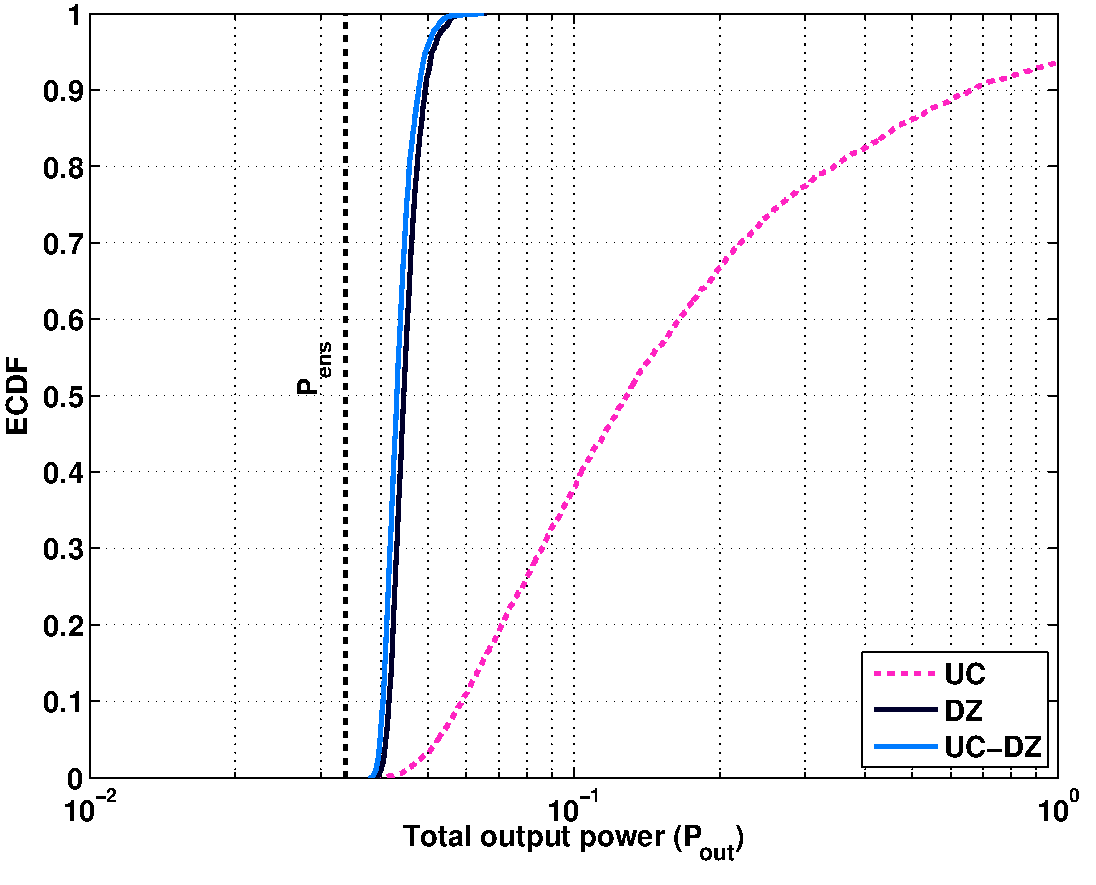
\includegraphics[width=3in]{dz_ucdz_ecdf_comp_single_interf.pdf}}
\subfloat[Multiple interferers]{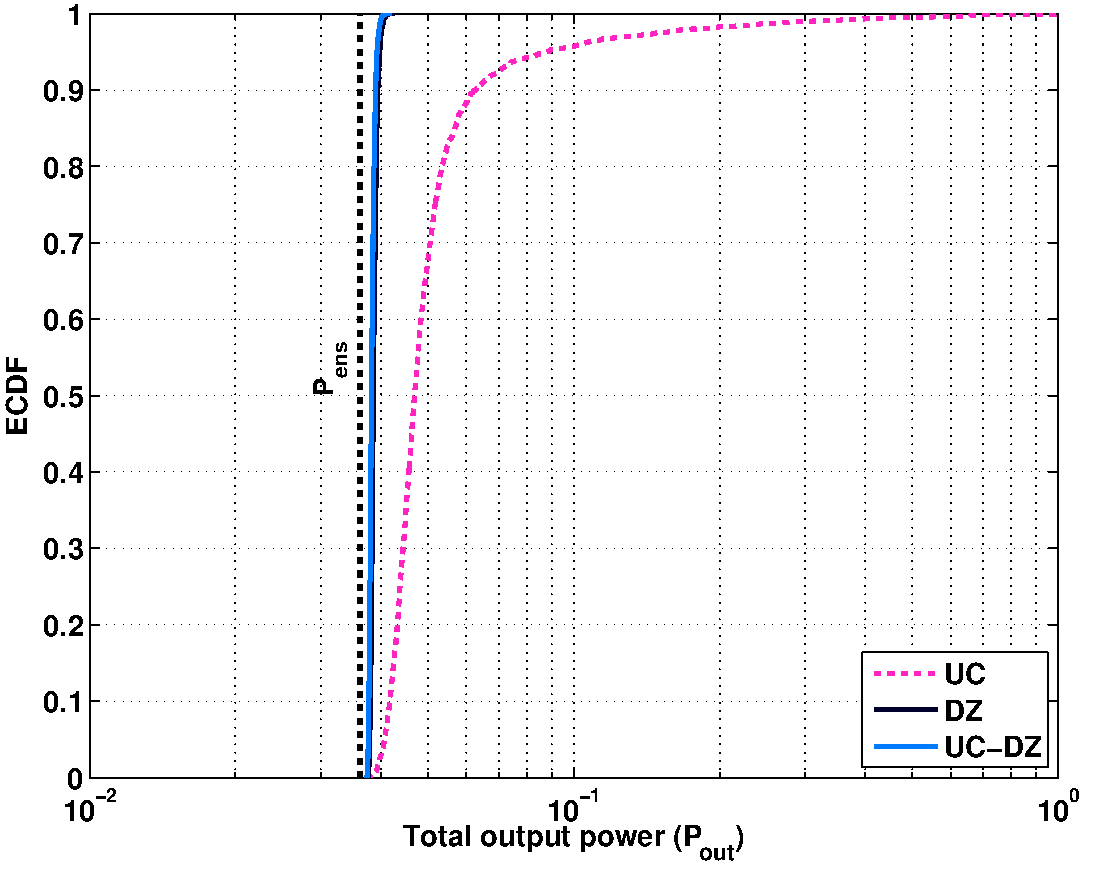
\includegraphics[width=3in]{dz_ucdz_ecdf_comp_multi_interf.pdf}}

\caption[Output power ECDF for the DZ MVDR, the unit circle UC
  constrained DZ MVDR and the UC MVDR ABF]{Output power ECDF for the DZ MVDR, the unit circle (UC)
  constrained DZ MVDR and the UC MVDR ABFs using an $N = 31$ element ULA
  and $L = 32$ snapshots. The UC constraint yields only a minimal gain
  over the DZ MVDR ABF.}
\label{fig:ecdf-dz-dzuc}
\end{figure}

% Multi interferer case: dz_ucdz_ecdf_comp_multi_interf

% THIS CAN GO INTO DISSERTATION
% % Mean var result discussion
% \figurename{}~\ref{fig:pout-mean-var-plots} compares the mean (solid) and
% variance (dashed) of the output power for the SMI MVDR ABF and the DZ MVDR
% ABF for the single interferer scenario, over a range of input INR levels
% from $0$ dB to $40$ dB. The DZ MVDR ABF produces output power with both lower
% mean and lower variance compared to the SMI MVDR ABF. The reduced mean output
% power demonstrates the DZ MVDR ABF's ability to suppress
% interferers. The reduced variance on output power suggests the DZ MVDR
% beamformer should achieve better detection performance as well.

% % Mean and var figure
% \begin{figure*}[!t]
%   \centering
%   \subfloat[$L = 32$]
%   {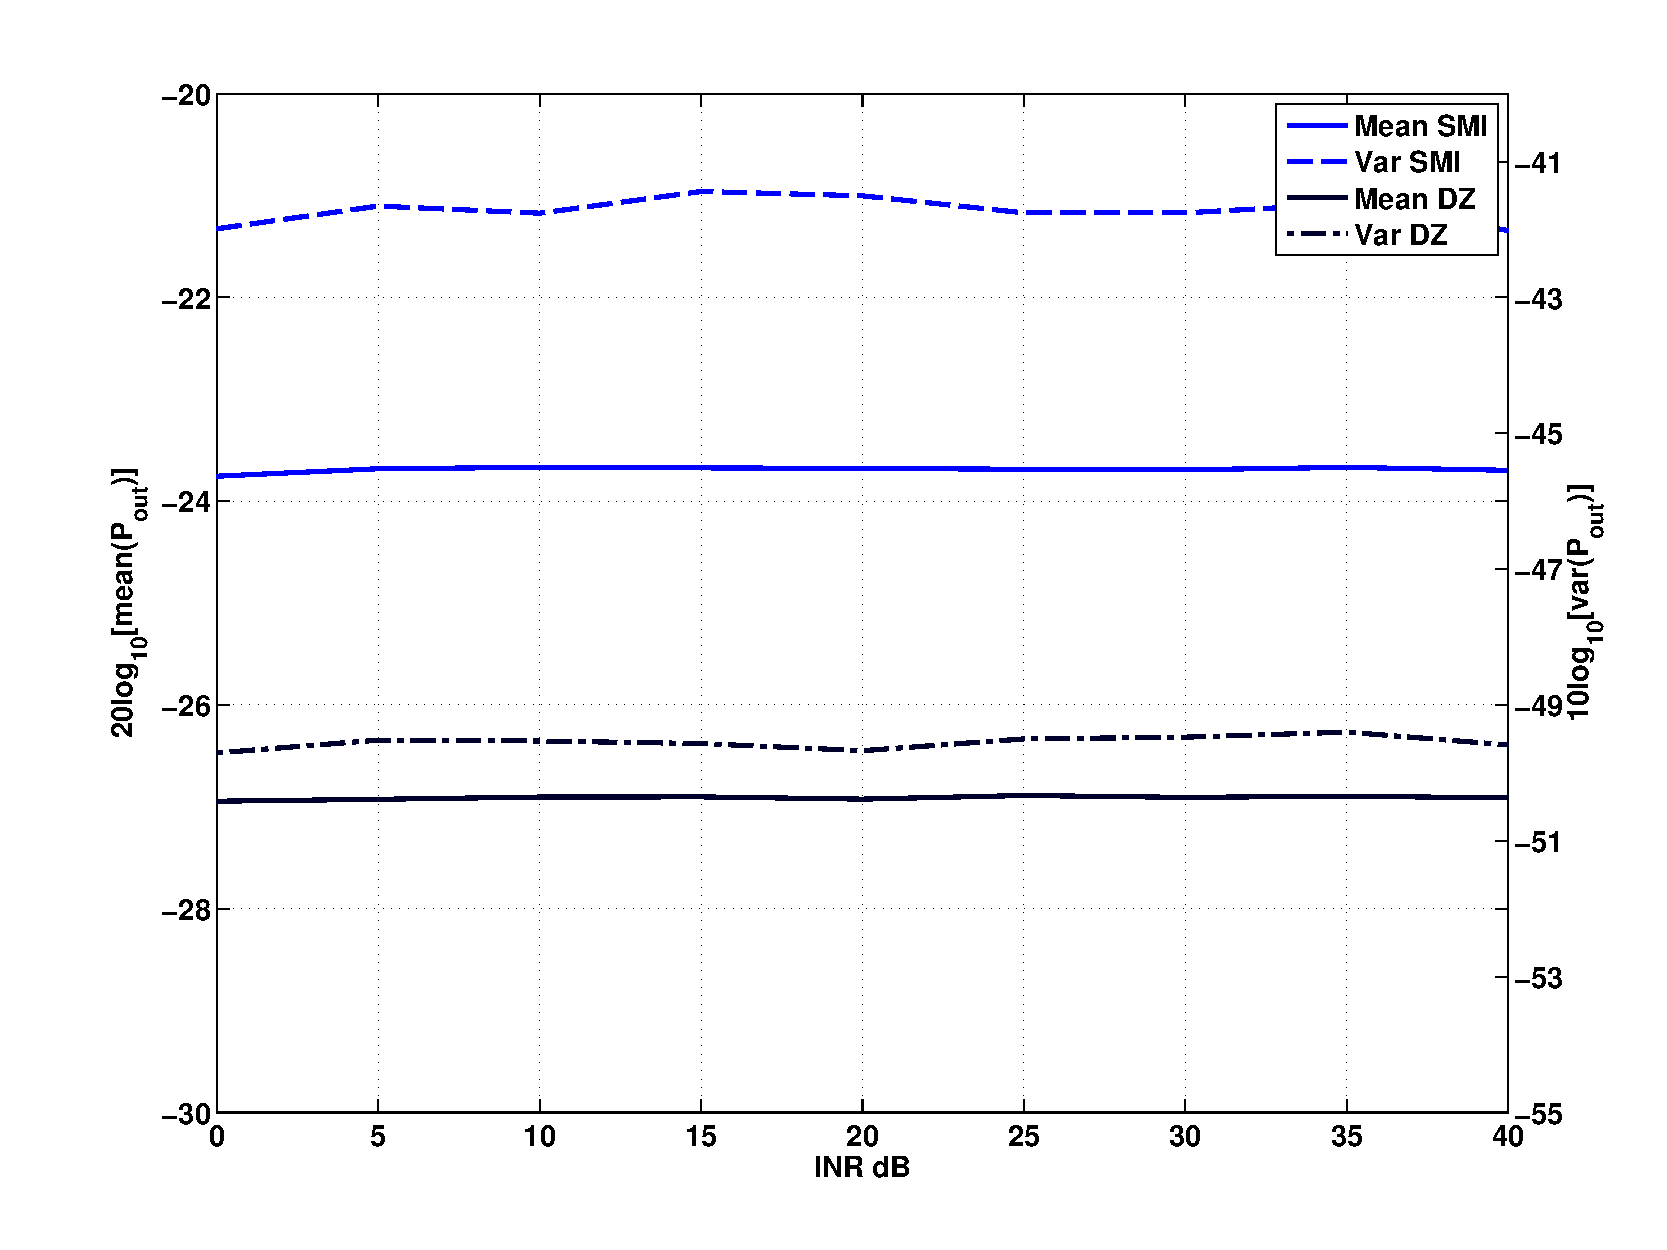
\includegraphics[width=2.8in]{mean_var_Pout_single_interf_N31_L62.pdf}
%     \label{fig:mean-var-single}}
%   \hfil
%   \subfloat[$L = 62$]
%   {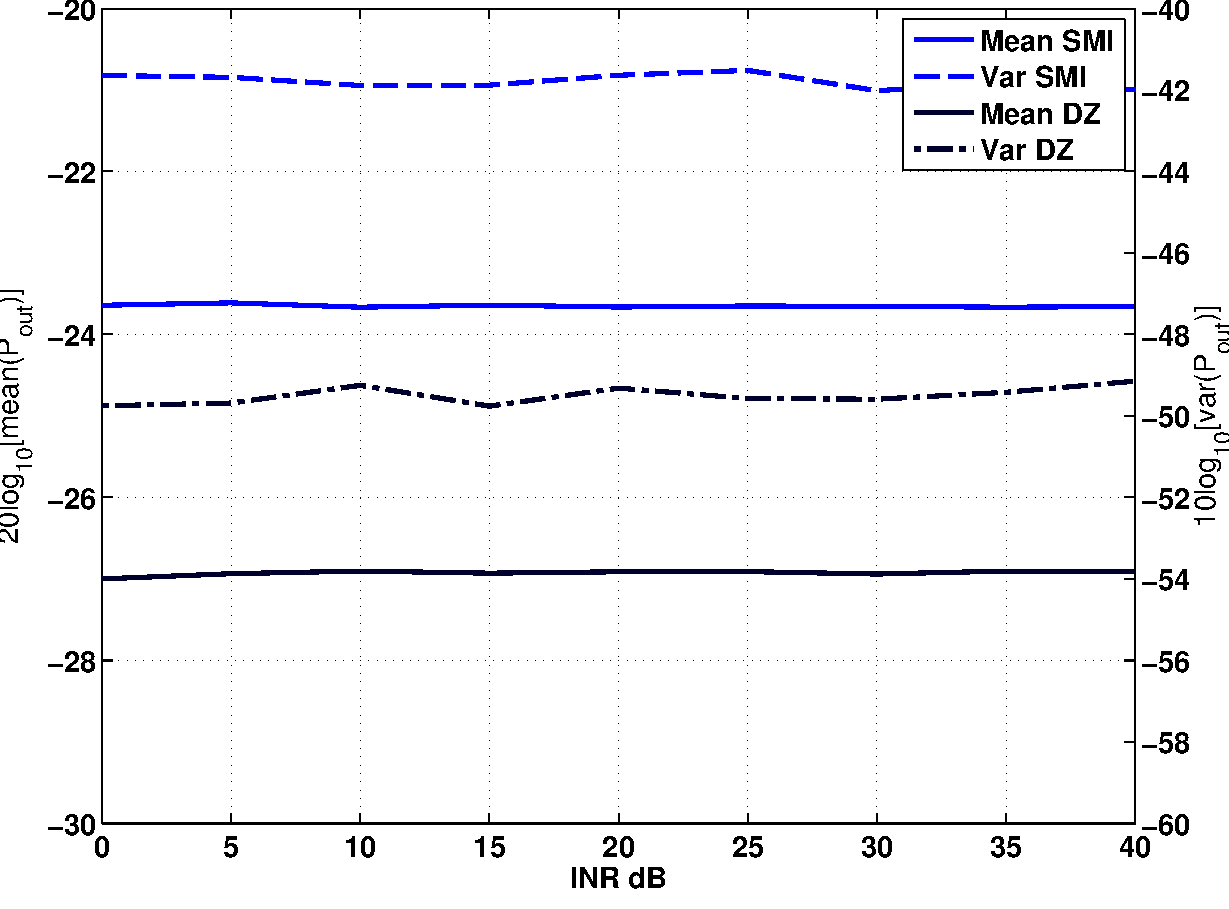
\includegraphics[width=2.8in]{mean_var_Pout_multi_interf_N31_L62.pdf}
%     \label{fig:mean-var-multi}}
%   \caption{Mean and variance of ABF output power over a range of input
%     INR for single interferer case. The DZ MVDR ABF output power has both lower mean and variance
%     compared to the SMI MVDR ABF.}
%   \label{fig:pout-mean-var-plots}
% \end{figure*}

% WNG discussion
\figurename{}~\ref{fig:wng-scatter} shows a scatter plot of the WNG
for the DZ MVDR and the SMI MVDR ABF. The top panel shows single
interferer scenario and the bottom panel shows the multiple interferer
scenario. In both plots, dot markers denote the snapshot limited case
($L = 32$) and the asterisk markers denote the snapshot sufficient
case ($L = 62$). Each dot and asterisk plots the WNG of the DZ MVDR
ABF against the WNG of the SMI MVDR ABF for one realization in the
Monte Carlo experiment. The optimal WNG for the experiment is $N = 31$
and the top right corner of the panel corresponds to the optimal WNG
for both ABFs \cite{vtree2002oap}. For all interferer scenarios and
snapshot conditions examined, the DZ MVDR ABF has better WNG than the
SMI MVDR ABF for almost every experimental trial. The DZ MVDR ABF
achieves consistently high WNG independent of the number of snapshots
for both the single and multiple interferer scenarios. In contrast,
the SMI MVDR ABF's WNG is very sensitive to the number of snapshots
available.  From the scatter plots, the DZ MVDR ABF exhibits higher
WNG on average compared to the SMI MVDR ABF. In addition to improving
the DZ MVDR ABF's ability to reject white background noise, the
improved WNG also indicates improved robustness against parameter
mismatch \cite{Gilbert1955}.

\begin{figure*}[!hp]
\centering
\subfloat[Single interferer]{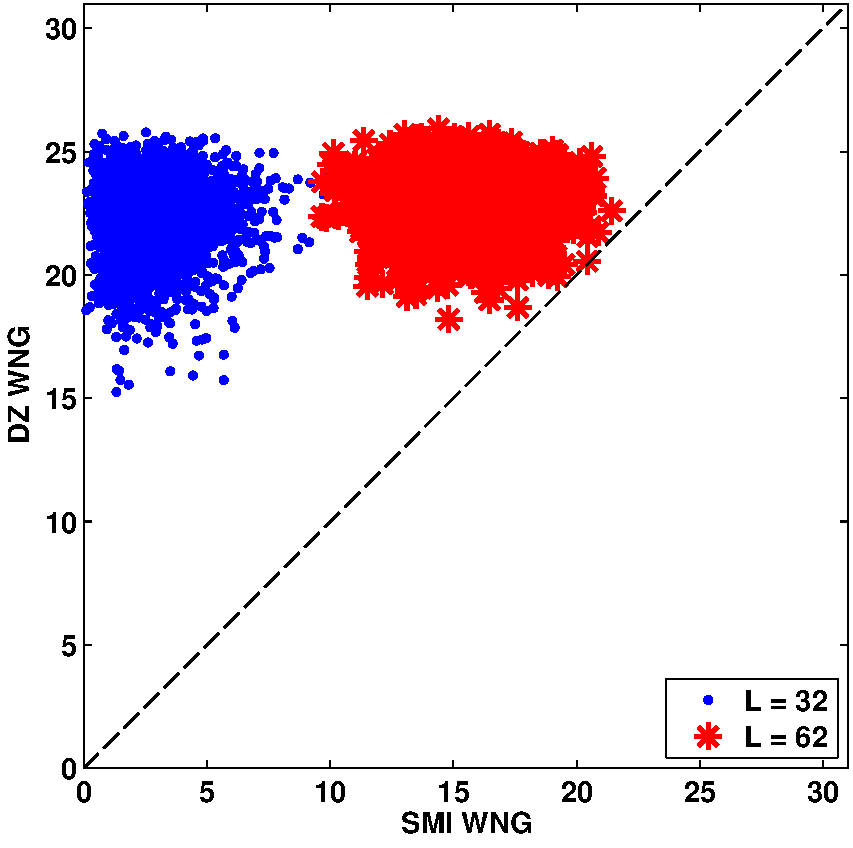
\includegraphics[width=3in]{wng_scatter_composite_single_N31.pdf}
%\subfloat[L = 32]{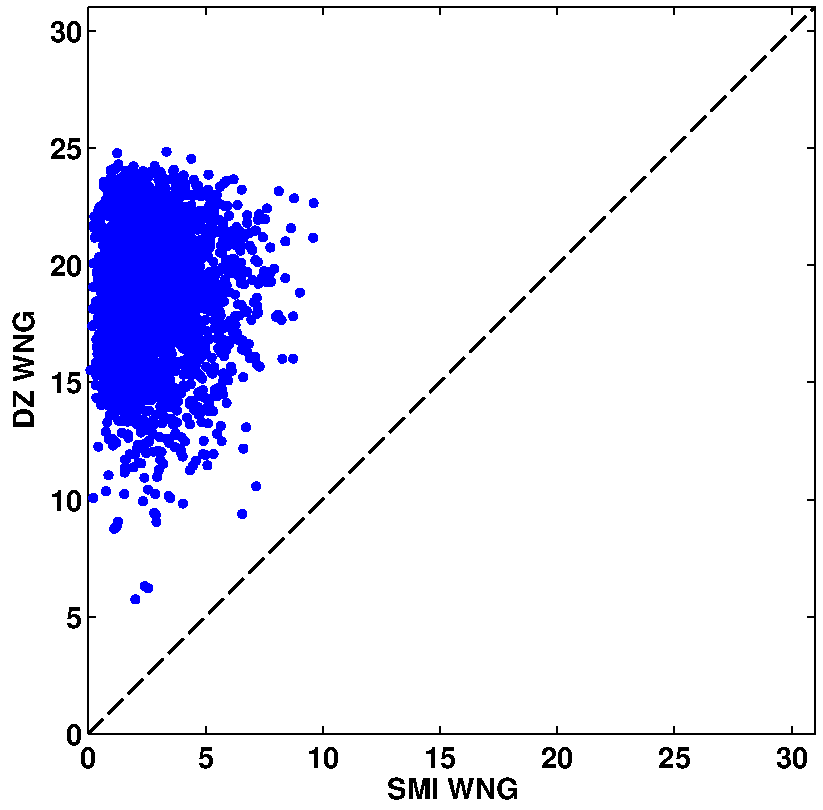
\includegraphics[width=2.5in]{wng_single_interf_N31_L32_INR40.pdf}
\label{fig:wng-s-L32}}

\subfloat[Multiple interferer]{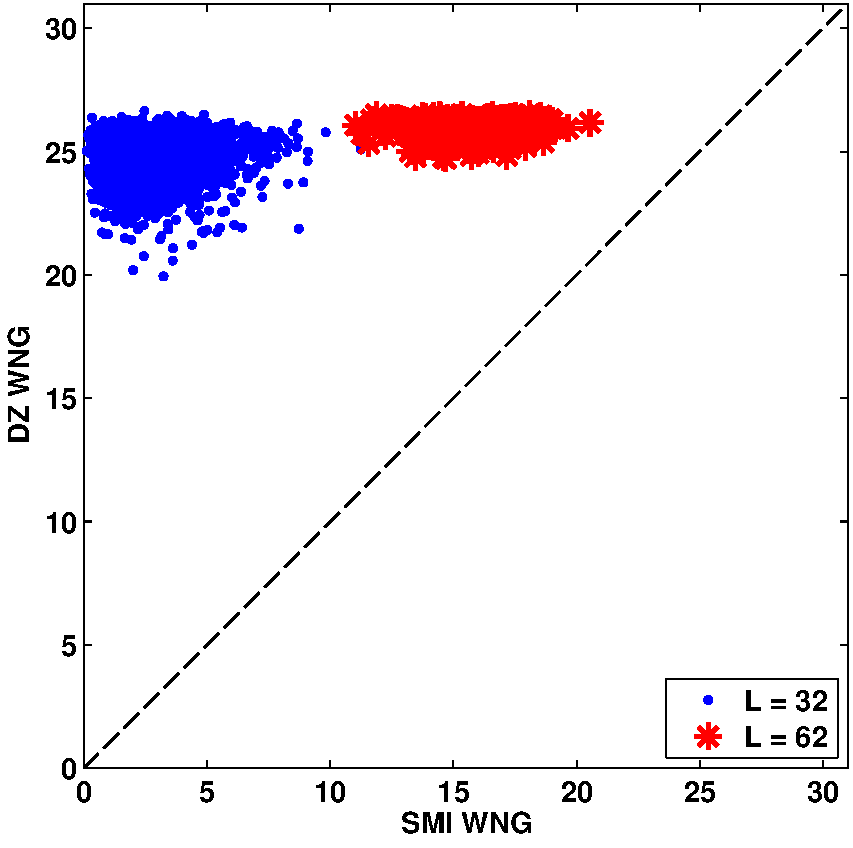
\includegraphics[width=3in]{wng_scatter_composite_multi_N31.pdf}
%\subfloat[L = 62]{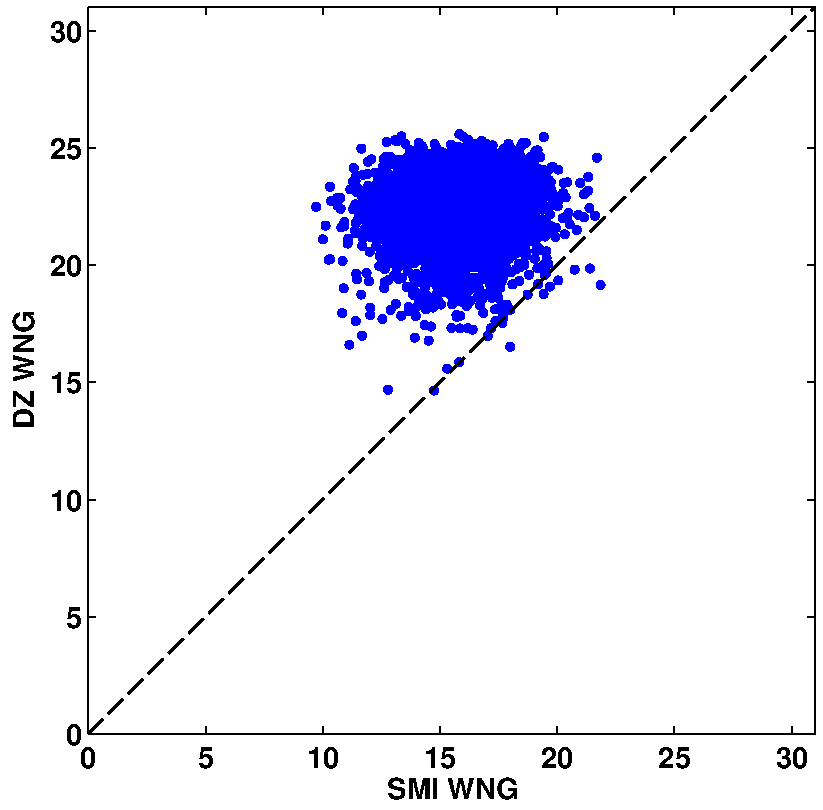
\includegraphics[width=2.5in]{wng_single_interf_N31_L62_INR40.pdf}
\label{fig:wng-s-L62}}
\caption[WNG scatter plot comparing the DZ MVDR and the SMI MVDR ABF]{WNG scatter plot comparing the DZ MVDR and the SMI MVDR ABFs
  using an $N = 31$ element ULA. On average, the DZ MVDR ABF has a
  higher WNG.}
\label{fig:wng-scatter}
\end{figure*}

% Output vs snapshot
\figurename{}~\ref{fig:pout-snapshot} compares the mean output power
between the DZ MVDR, the SMI MVDR, and the DL MVDR ABFs for
implementations using $L = [32, 48, 62]$ snapshots. The top panel
shows the single interferer scenario and the bottom panel shows the
multiple interferer scenario. In both panels, the solid horizontal
line denotes the ensemble MVDR output power. For both interferer
scenarios and all snapshot cases, comparisons show that the DZ MVDR ABF
produces consistently lower mean output power compared to the SMI MVDR
ABF. When snapshot rich ($L = 62$), the DZ MVDR ABF output power is
lower than the SMI MVDR ABF output only by a factor less than two in
both the single and the multiple interferer scenarios. But when
snapshot limited ($L = 32$) the DZ MVDR ABF mean output power is lower
than the SMI MVDR ABF mean output power by a factor more than ten. As
mentioned previously, the decrease in the number of snapshots results
in an increased interferer direction mismatch. The mismatch leads to the
loss of interferer suppression for the SMI MVDR ABF and produces
higher output power. At the same time, the DZ MVDR ABF with its
broader notches is robust against the interferer direction
mismatch. The broader notches consistently suppress the interferers to
produce lower mean output power compared to the SMI MVDR ABF.

In the experiment, for both interferer scenarios and each snapshot
case, the DL factor for the DL MVDR ABF is chosen to match the average
WNG between the DL MVDR and the DZ MVDR ABFs. Hence the two ABFs have
comparable white noise power suppression. In
\figurename{}~\ref{fig:pout-snapshot}, comparisons between the DZ MVDR
and the DL MVDR ABFs shows that they have essentially same output
power performance for all cases in both interferer scenarios. This
implies that the output power is dominated by white noise contribution
and the interferer power contribution is negligible. Both the DZ MVDR
and the DL MVDR ABFs suppress the interferer power significantly
better compared to the SMI MVDR ABF. However, the approach used to
choose WNG in the experiment is not realistic as it requires
iteratively solving for the DL factor to match the average WNGs. In
practice the DL MVDR ABF still requires choosing a DL factor, while
the DZ MVDR ABF does not require setting a design parameter prior to
implementation. On the other hand, the DL MVDR ABF can in principle
handle more than $N/2$ interferers, while the DZ MVDR ABF is limited
to to about $N/2$ interferers due to the subarray approach
constraining the number of degrees of freedom.

\begin{figure*}[!hp]
\centering
\subfloat[Single interferer]{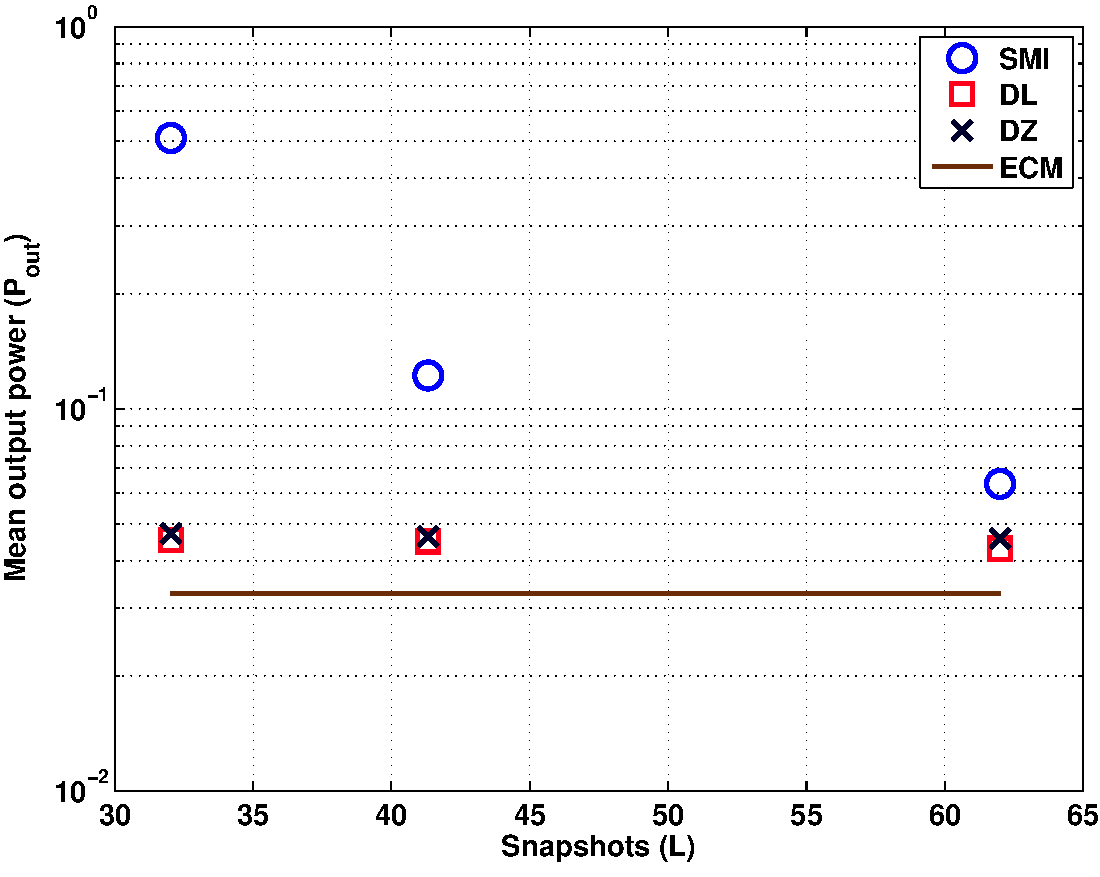
\includegraphics[width=3.5in]{pout_snapshot_N31_single.pdf}
\label{fig:pout-snapshot-L32}}
\hfil
\subfloat[Multiple interferers]{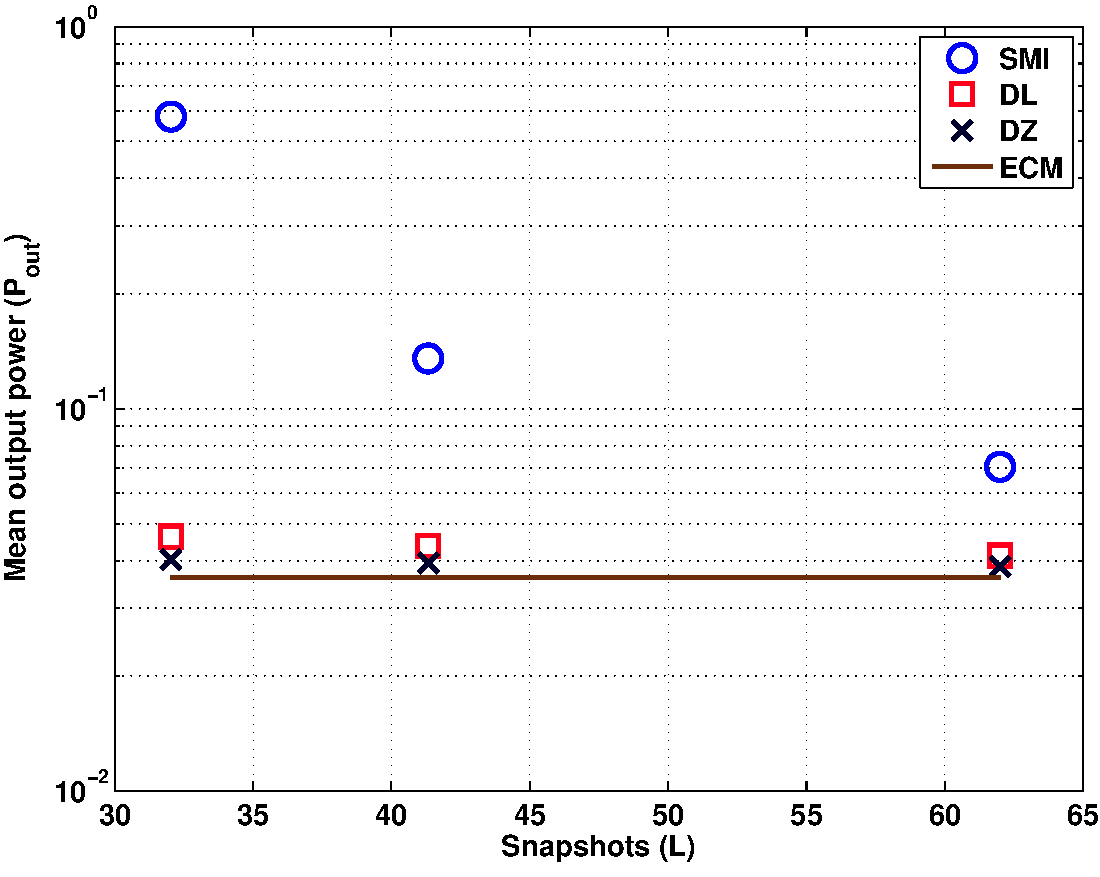
\includegraphics[width=3.5in]{pout_snapshot_N31_multi.pdf}
\label{fig:pout-snapshot-L62}}
\caption[Mean output power from ABFs using different number of
snapshots for single and multiple interferer cases]{Mean output power
  from ABFs using different number of snapshots for single and
  multiple interferer cases. The DZ MVDR ABF exhibits significant gain
  over the SMI MVDR ABF in suppressing output power when snapshot
  limited. The DZ MVDR ABF has a mean output power comparable with the
  DL MVDR ABF.}
\label{fig:pout-snapshot}
\end{figure*}

% The inherent subarray processing involved in implementing the DZ MVDR
% ABF widens the main lobe width and limits the degree-of-freedom
% available to suppress interferers to $(N - 1)/2$. But the results
% above indicate that the DZ MVDR ABF is still capable of reducing the 
% output power in presence of multiple interferers compared to the
% traditional SMI MVDR ABF. The consequences of subarray processing is
% further minimized in underwater applications where it is
% common to use long ULAs with hundreds of sensors
% \cite{baggeroer1999passive}. 

\subsection{Moving interferer case} 
\label{sec:moving-interferer}
This section presents results from numerical experiments evaluating
the performance of the ABFs in a moving interferer scenario. The
experiment assumes a scenario containing single spatially moving
interferer in a white background noise similarly to the
example in \cite[Sec. 4]{cox2000mrabf}. The interferer is initially at
direction $u_0 = 5/N$ and moves away from the main lobe at a constant
rate of $\rho_u$ per snapshot. The interferer direction at the
$l^{th}$ snapshot index is $u_l = u_0 + (l-1) \rho_u $ for
$l = 1, \ldots, L$ and $\rep_l = \rep(u_l)$ is the array manifold
vector for the $l\nth$ snapshot. During the snapshot averaging
interval ($l = 1,\ldots, L$), the interferer traverses some fraction
($\mu$) of the ULA resolution width, i.e.,
$\mu = \rho_u (L-1)(N - 1)/2$.

The results compare the output power of the ABFs for
varying interferer velocity cases. In each velocity case, same
number of snapshots $L = 32$ are used to estimate the SCM and compute
the weight vector ($\wthat$) for each ABF. The experiment assumes an
inbred processing approach, where the ABF weights are applied to the
same data used to compute the weights \cite{cox2002adaptive}. Several
other approaches exist for processing data in a non-stationary
environment. However, in order to make a fair comparison between the
ABFs, the experiment uses one consistent approach for all of the ABFs
compared.

In order to evaluate the ABF's output power in the moving interferer
scenario, define a `time averaged' ECM
\begin{align}
  \label{eq:time-avg-ecm}
  \avgCov &= (\interfpow/L)\sum_{l = 1}^{L}\rep_l\rep_l^H +
            \noisepow\eye  \nonumber \\ 
  &= \interfpow\repmat_L\repmat_L\herm + \noisepow\eye,
\end{align}
where $\repmat_L$ is an $N\times L$ matrix of $L$ array manifold
vectors corresponding to the interferer direction $u_l$ at each
snapshot index $l$. The `time averaged' ECM defined in
\eqref{eq:time-avg-ecm} is equivalent to an ECM corresponding to a
scenario containing $L$ independent sources each in the direction $u_l$
with power $\interfpow/L$. This scenario is essentially how the moving
interferer appears to the ULA over the snapshot averaging window
assuming perfect knowledge of the environment. The `time averaged'
ECM captures the interferer motion during the snapshot averaging
window of $l = 1,\ldots, L$. An MVDR beamformer implemented using the
'time averaged' ECM attempts to place a deep notch in each of the $L$
directions ($u_l$).

In the results discussed below, a single realization of the ABF output
power is evaluated as $\pout = \wthat\herm\avgCov\wthat$ where
$\wthat$ is the ABF weight vector. Using the definition of the `time
averaged' ECM in \eqref{eq:time-avg-ecm} the output power is,
\begin{align}
  \label{eq:time-avg-pout}
  \pout &= (\interfpow/L)\wthat\herm\repmat_L\repmat_L\herm\wthat + \noisepow\norm{\wthat}^2 \nonumber \\
&= \pinter + \pnoise,
\end{align}
where $\pinter$ is the output interferer power and $\pnoise$ is the
output noise power. All the results are obtained from a 3000 trial
Monte Carlo experiment assuming the moving interferer with $30$dB INR
and unit power white noise ($\noisepow = 1$). The CMT MVDR ABF is
implemented using the notch width parameter $\cmtW = \resW$.

\figurename{}~\ref{fig:moving-interf-ecdf} compares the output power
ECDF of the DZ MVDR, the CMT MVDR and the SMI MVDR ABFs for the moving
interferer scenario described above. The top panel assumes the
interferer traverses one resolution width during snapshot averaging
($\mu = 1$) and the bottom panel assumes the interferer moves two
resolution widths during snapshot averaging ($\mu = 2$). The dotted
vertical lines on both panels denote the output power from the
ensemble MVDR implemented using the `time averaged' ECM $\Cov_A$. This is the minimum output power achievable using the processing scheme of computing weights from $L$ snapshots. Comparisons
in \figurename{}~\ref{fig:pout-ecdf-mu1}, the case of $\mu = 1$, show
that the DZ MVDR ABF has higher probability of minimizing the output
power compared to the SMI MVDR ABF. The median output power of the DZ
MVDR ABF is more than eight times lower compared to the SMI MVDR ABF.
Also, the ECDF of the DZ MVDR ABF rises faster compared to the ECDF of
the SMI MVDR ABF indicating the output power of the DZ MVDR ABF
exhibits less variability than the output power of the SMI MVDR
ABF. The CMT MVDR ABF also improves performance over the SMI MVDR
ABF. But the DZ MVDR ABF still achieves lower median output power
compared to the CMT MVDR.

Comparisons in \figurename{}~\ref{fig:pout-ecdf-mu2}, the case of
$\mu = 2$, show that the DZ MVDR ABF again has higher probability of
minimizing the output power compared to both the SMI MVDR and the CMT
MVDR ABF. In this case, the interferer is moving at twice the velocity
compared to the case of $\mu = 1$. But the CMT MVDR ABF is still
implemented using the width parameter $\cmtW = 2/N$. The increased
interferer velocity elevates the interferer mismatch problem compared
to the case in \figurename{}~\ref{fig:pout-ecdf-mu1}. Comparing the
two velocity cases, the DZ MVDR ABF median output power increases with
the velocity while the CMT MVDR and the SMI MVDR ABFs have negligible
change in output power.

\begin{figure*}[!hp]
\centering
\subfloat[$\mu = 1$]
{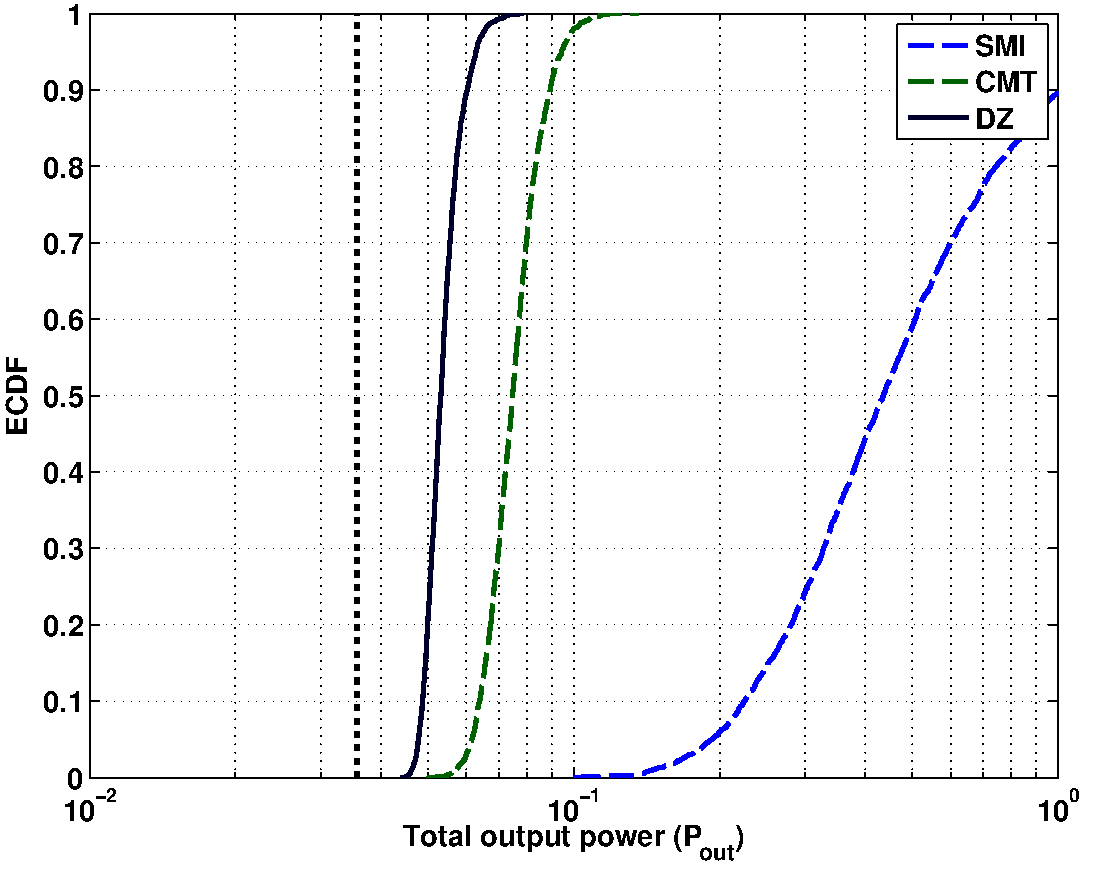
\includegraphics[width=3.5in]{dzmv_moving_interf_pout_ecdf_mu1.pdf}
\label{fig:pout-ecdf-mu1}}

\subfloat[$\mu = 2$]
{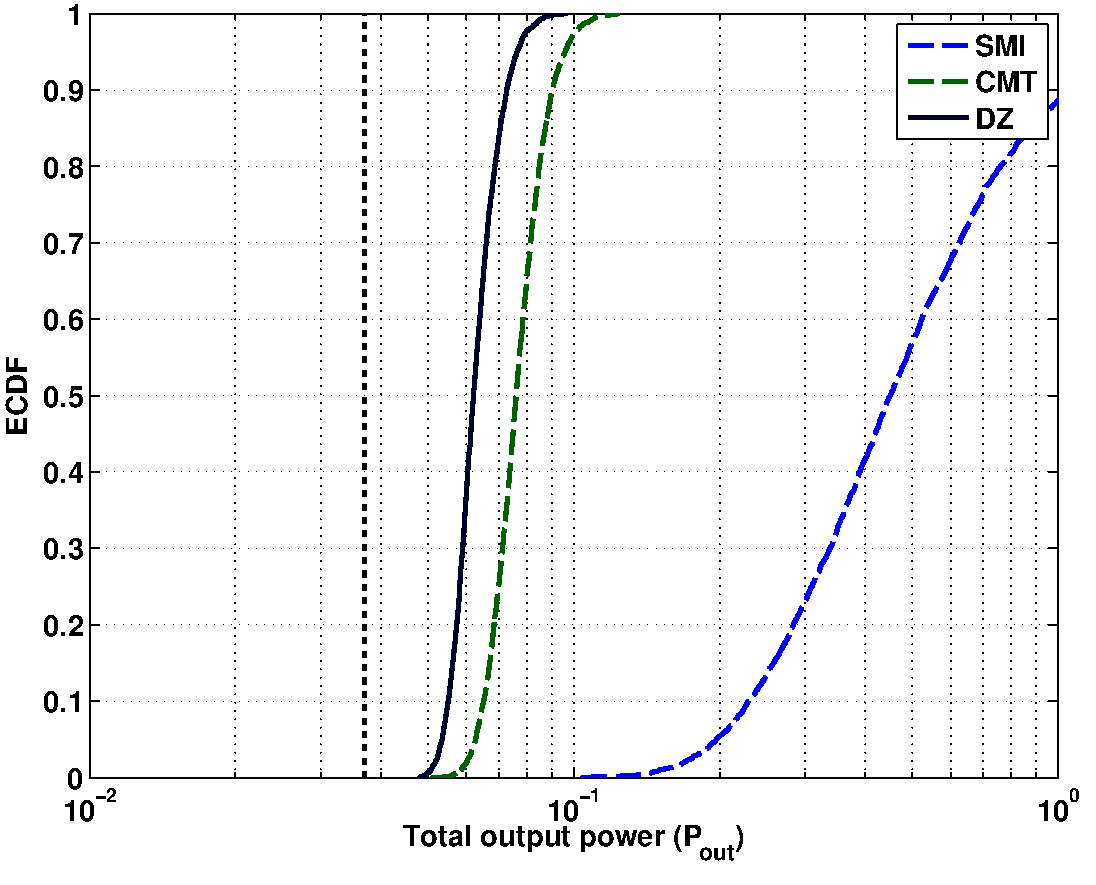
\includegraphics[width=3.5in]{dzmv_moving_interf_pout_ecdf_mu2.pdf}
\label{fig:pout-ecdf-mu2}}
\caption[Total output power ECDF for the DZ MVDR, the CMT MVDR and the
SMI MVDR ABFs for different interferer velocity cases]{Total output
  power ECDF for the DZ MVDR, the CMT MVDR and the SMI MVDR ABFs using
  an $N = 31$ element ULA for two interferer velocity cases ($\mu = 1$
  and $\mu = 2$). The DZ MVDR ABF has higher probability of minimizing
  output power compared to both the SMI MVDR and the CMT MVDR ABF. }
\label{fig:moving-interf-ecdf}
\end{figure*}
\figurename{}~\ref{fig:varying-velocity} compares the outputs from the
DZ MVDR (black diamonds), the CMT MVDR (green squares) and the SMI
MVDR ABF (blue circles) for different interferer velocity cases.  The
top panel shows the interferer contribution to output power
($\pinter$), the middle shows the white noise contribution to output
power ($\pnoise$) and the bottom panel shows the total output power
($\pout$). Since the noise power is assumed to be unity, the noise
contribution to the output power is simply equal to the reciprocal of
the WNG as shown in \eqref{eq:time-avg-pout}.

The experiment evaluates the ABFs for cases when the interferer
traverses $\mu = \{0.5, 1, 2, 3, 4\}$ fraction of resolution width
during $L = 32$ snapshot averaging window. The interferer
contribution, the noise contribution and the total output power is
evaluated as defined in \eqref{eq:time-avg-pout} for each velocity
case. For all velocity cases, the CMT MVDR ABF is implemented with
$\cmtW = 2/N$.

\begin{figure*}[!hp]
\centering
\subfloat[Interferer output power]
{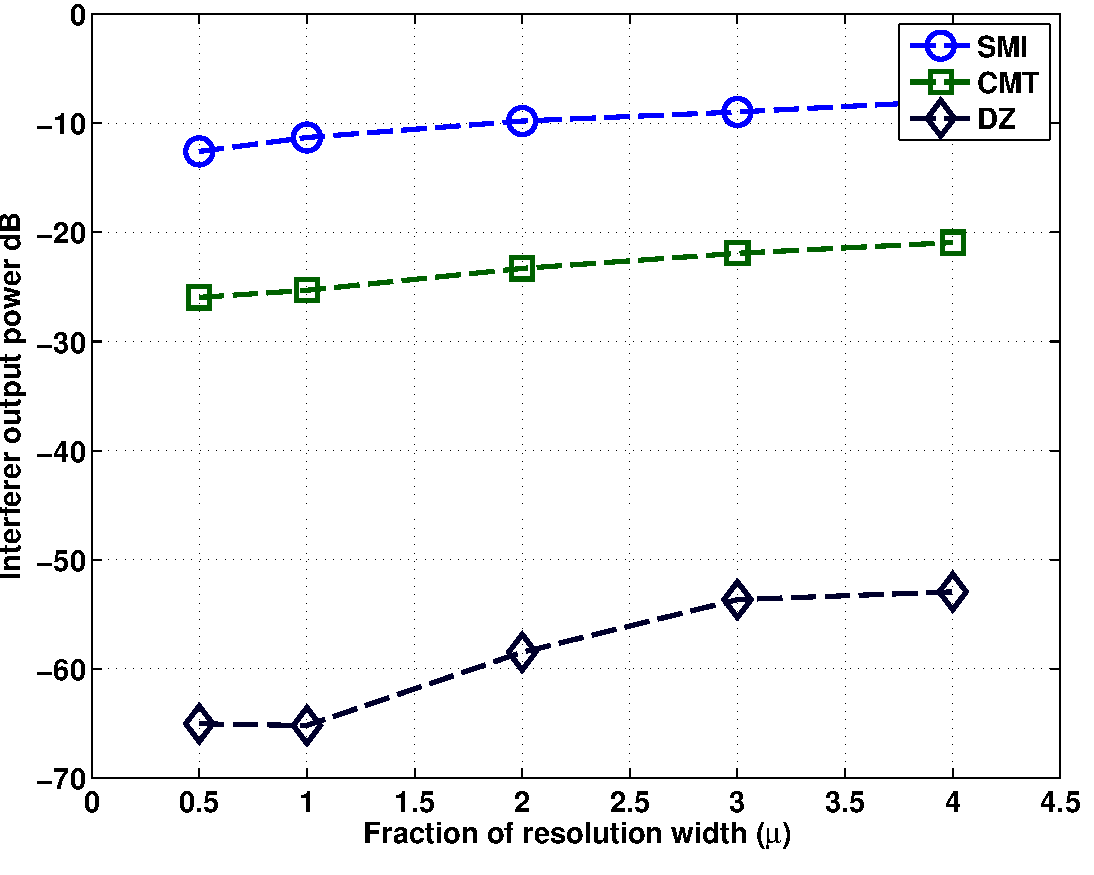
\includegraphics[width=3in]{interf_pout_diff_motion.pdf}\label{fig:interfp-diff-vel}}
\subfloat[WNG]
{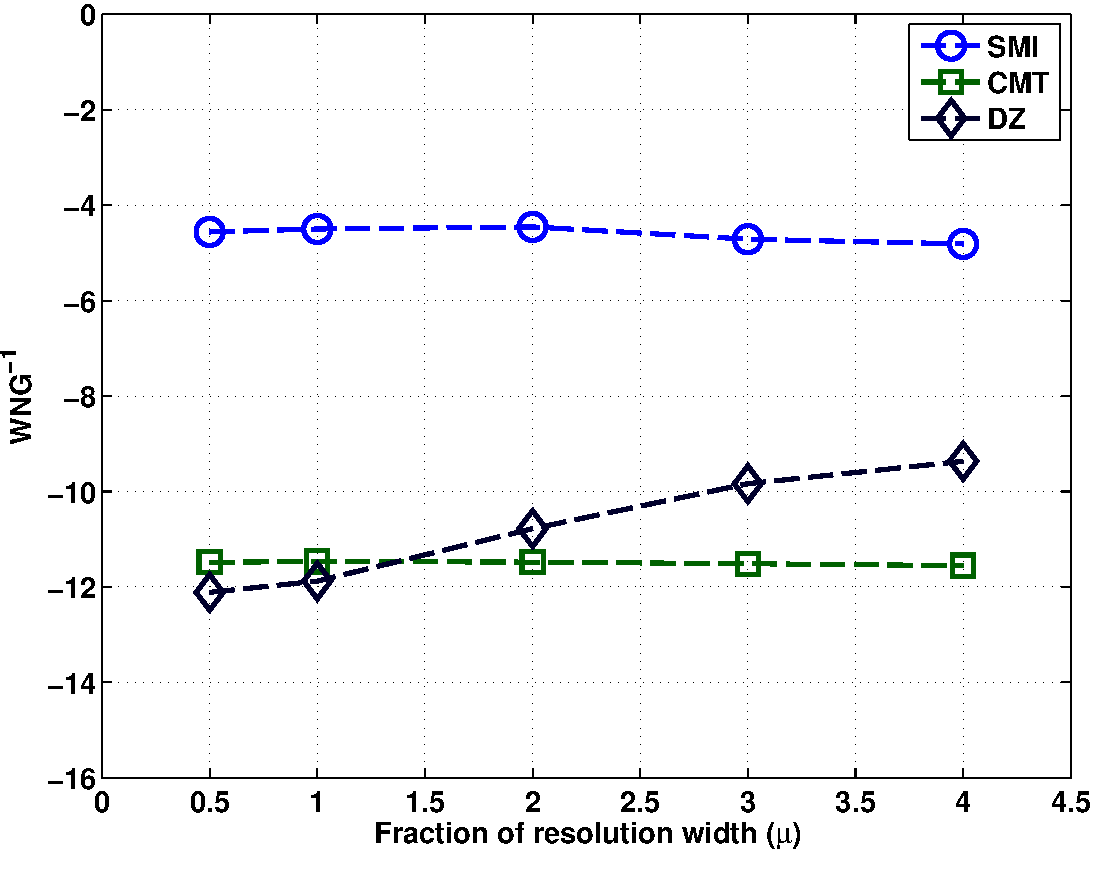
\includegraphics[width=3in]{wng_diff_motion.pdf}\label{fig:wng-diff-vel}}

\subfloat[Total output power]
{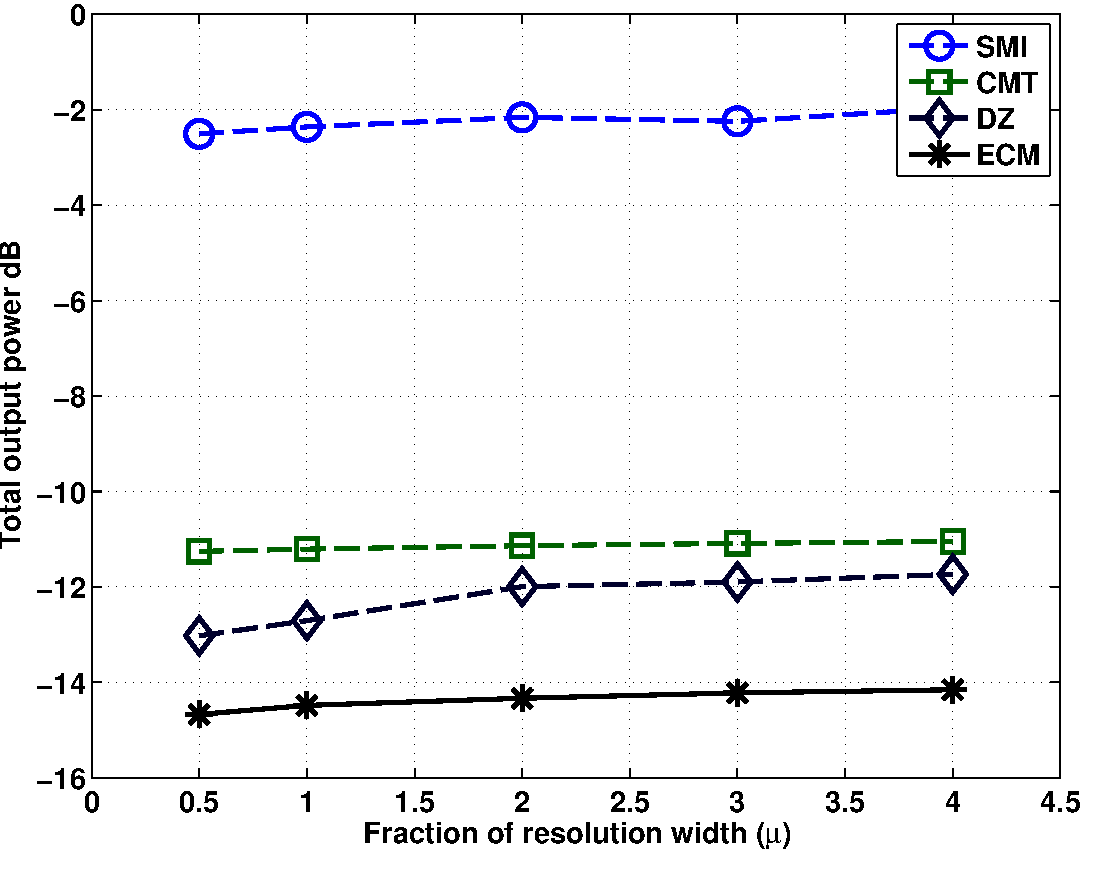
\includegraphics[width=3in]{mean_pout_diff_motion.pdf}\label{fig:outp-diff-vel}}

\caption[Output from the DZ MVDR, the SMI MVDR, and the CMT MVDR ABFs
using for varying interferer velocity cases]{Output from the DZ MVDR,
  the SMI MVDR, and the CMT MVDR ABFs using an $N = 31$ element ULA
  for varying interferer velocity cases. The mean output power of the
  DZ MVDR ABF is about $10$dB below the SMI MVDR ABF for all velocity
  cases. The mean output power of the DZ MVDR ABF is comparable with
  that of the CMT MVDR ABF.}
\label{fig:varying-velocity}
\end{figure*}


\figurename{}~\ref{fig:interfp-diff-vel} compares the mean interferer output power for each ABF at all velocity cases. Comparison shows the DZ MVDR ABF
suppresses interferers significantly better than the SMI MVDR ABF for
all velocity cases. The mean interferer output power for the DZ MVDR
ABF is more than $40$ dB below that of the SMI MVDR ABF in all
velocity cases. Comparatively, the mean interferer output power for
the CMT MVDR ABF is only about $10$ dB below that of the SMI MVDR ABF
in all velocity cases. As mentioned earlier, the DZ MVDR ABF reduces
the estimation bias of interferer eigenvectors as a consequence of
inherent subarray processing. Thus the DZ MVDR ABF is able to create
broader and deeper notch at the interferer and yield better
improvement in interferer suppression compared to the CMT MVDR ABF in
all cases of the experiment.

\figurename{}~\ref{fig:wng-diff-vel} compares the white noise
contribution to output power for each ABF at all velocity cases. The
solid horizontal line denotes the noise output power corresponding to
the optimal WNG of $N = 31$. Comparison shows that the DZ MVDR ABF has
better WNG compared to the SMI MVDR ABF and hence lower output noise
power for all velocity cases. When the interferer motion is limited
within the resolution width ($\mu \leq 1$), the DZ MVDR ABF yields
highest WNG and the lowest output noise power. At higher velocities
($\mu \geq 2$), the DZ MVDR and the CMT MVDR ABF both have comparable
output noise power. 

\figurename{}~\ref{fig:outp-diff-vel} compares the mean total output
power for each ABF at all velocity cases. The black asterisk markers
denote the output power from the ensemble MVDR implemented using the
`time averaged' ECM. The total output power is the combination of
interferer output power and the noise output power. In all velocity
cases, the contribution from the white noise dominates the total
output power for the DZ MVDR and the CMT MVDR ABFs. Both the DZ MVDR
and the CMT MVDR ABF yield significantly lower mean output power
compared to the SMI MVDR ABF in all moving interferer scenarios.
However, the CMT MVDR ABF requires choosing the notch width
parameter while the DZ MVDR ABF does not require setting a design
parameter to produce comparable performance.

\subsection{CMT MVDR ABF with multiple interferers}
\label{sec:cmt-multi-interf}
The CMT MVDR ABF with notch width $\cmtW = 2/(N-1)$ uses three degrees
of freedom (DoF) per interferer to produce broad notch as discussed in
\sect{}~\ref{sec:cmt}. The DZ MVDR ABF by design uses two DoF per
interferer. This section compares the output performance of the CMT
MVDR and the DZ MVDR ABF in case of a multiple interferers scenario.

\figurename{}~\ref{fig:cmt-output-multi} compares the average output
power from the DZ MVDR (black diamonds) and the CMT MVDR ABF (green
circles) for four cases with number of interferers
$D = \lbrace 1, 2, 3, 4 \rbrace$ respectively. The experiments starts
with $D = 1$ interferer at $\uinter = -7/N$ and introduces one
additional interferer for each new case. The direction for additional
interferers is chosen sequentially from the set
$\mathbf{\uinter} = \lbrace 7/N,~3/N,~-3/N \rbrace$ respectively. For
all four cases, both ABFs are implemented using an $N = 11$ element
ULA and steered towards broadside ($\ulook = 0$). The CMT MVDR ABF is
implemented using notch width $\cmtW = 2/(N - 1$).  Examining the
output power, the DZ MVDR and the CMT MVDR ABF produce comparable
output for $ D \leq 2$. But for $D > 2$, the CMT MVDR ABF produces
significantly higher output power compared to the DZ MVDR ABF.
\figurename{}~\ref{fig:wng-cmt-multi} compares the inverse of the WNG
of the ABFs.  The inverse of WNG is proportional to the white noise
contribution to output power. When $D > 2$ the white noise
contribution of the CMT MVDR ABF increases significantly. In the
presence of multiple interferers, the CMT MVDR ABF fails to suppress
output power as it uses more DoF per interferer compared to the DZ
MVDR ABF as discussed below.

The MVDR ABFs using the $N = 11$ element ULA and steered to a fixed
look direction are limited to $N-2 = 9$ DoF for adaptation. When
$D = 2$, the CMT MVDR uses six DoF to suppress interferer and the
remaining DoFs are used for white noise suppression. But when $D = 3$,
the CMT MVDR ABF uses all nine DoF to suppress interferer leaving no
DoF for white noise suppression. This results in loss of WNG for the
CMT MVDR and subsequent increase in white noise contribution to output
power. Moreover when $D = 4$, the CMT MVDR ABF requires more than nine
DoF, which results in failure to suppress interferer and loss of
WNG. As a result the CMT MVDR ABF produces significantly high output
power. In contrast, even when $ D = 4$, the DZ MVDR uses only eight
DoF to suppress interferers leaving the remaining DoF for white noise
suppression. Hence the DZ MVDR ABF consistently produces lower output
power in all four interferer cases.

\begin{figure*}[!hp]
  \centering
  \subfloat[Total output power]{    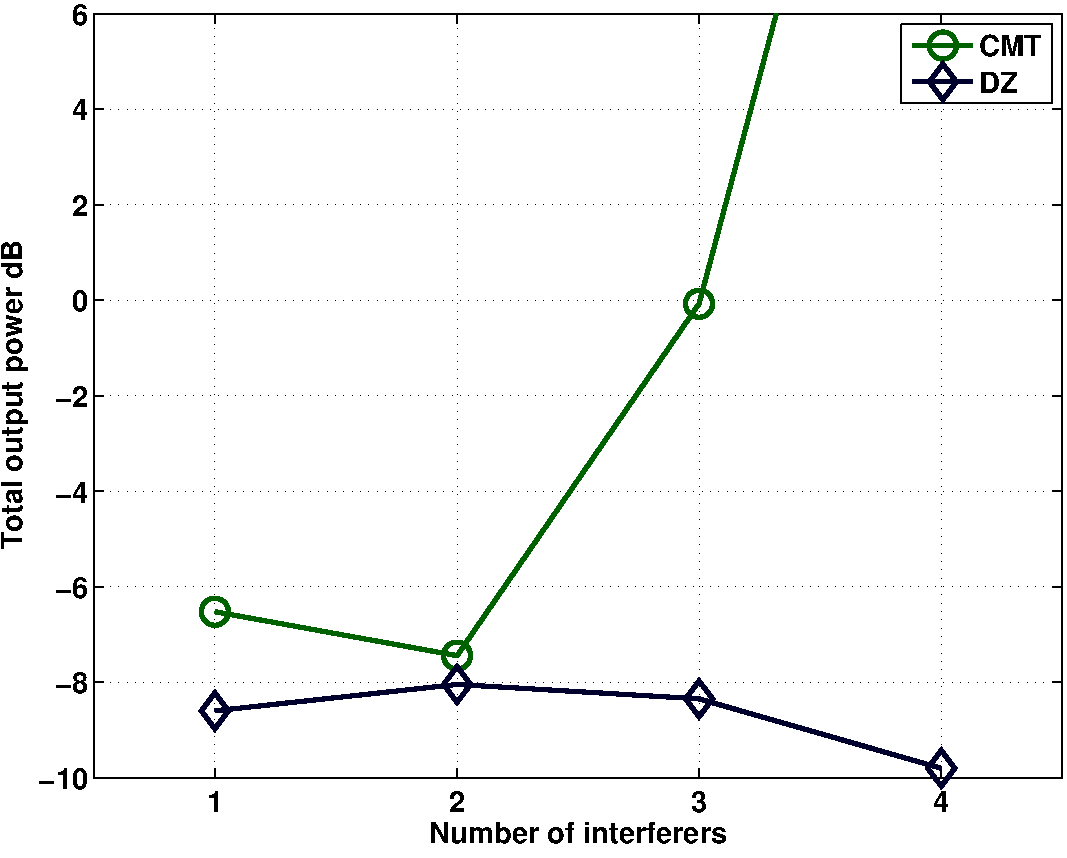
\includegraphics[width=3.5in]{./cmt_multi/dz_vs_cmt_Pout_multi_case2.pdf}
    \label{fig:cmt-output-multi}}

  \subfloat[White noise contribution]{
    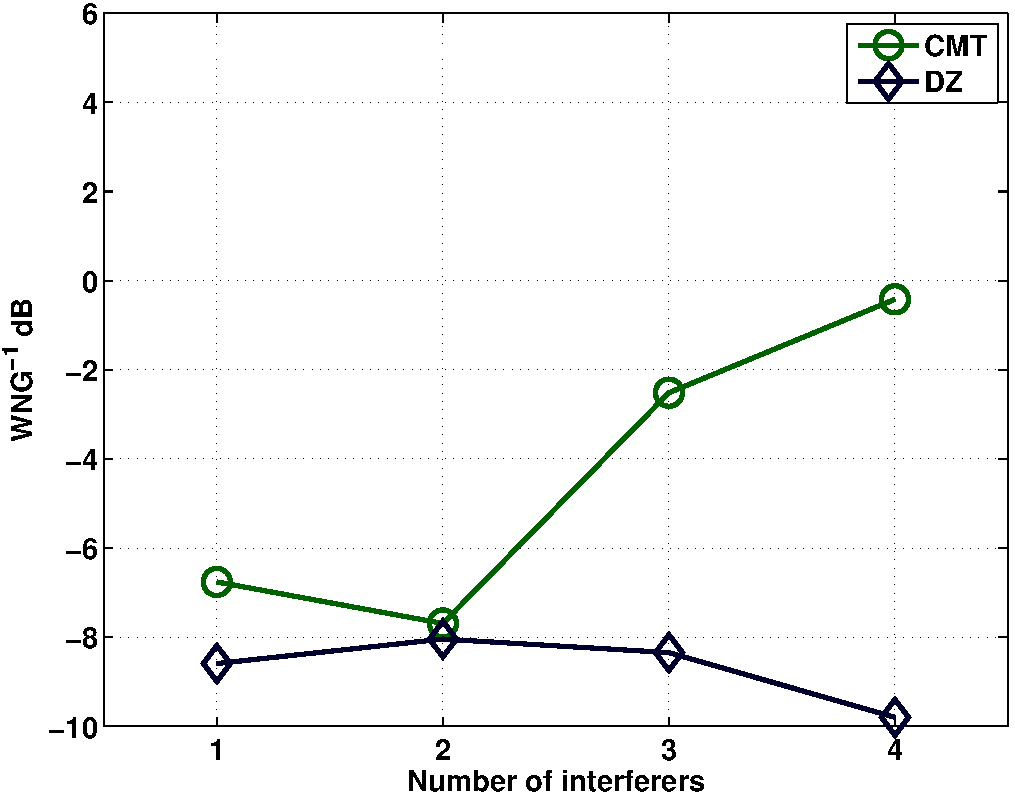
\includegraphics[width=3.5in]{./cmt_multi/dz_vs_cmt_wng_multi_case2.pdf}
    \label{fig:wng-cmt-multi}}
  \caption[Comparison of output from the DZ MVDR and the CMT MVDR ABFs for
    different number of interferers]{Comparison of (a) Output power and (b) white noise
    contribution to output from the DZ MVDR and the CMT MVDR ABFs for
    different number of interferers. Both ABFs are implemented using
    $N = 11$ sensor ULA and steered towards broadside. The CMT MVDR
    uses notch width of $\cmtW = 2/(N-1)$. As the number of
    interferers increases, the CMT MVDR fails to suppress output power
    as it uses more DoF per interferer compared to the DZ MVDR ABF.}  
\end{figure*}

% As previously mentioned, the DZ MVDR ABF has only $(N-1)/2$ degrees of
% freedom (DoF) for interferer suppression. Equivalently the DZ MVDR
% polynomial has only $(N-1)/2$ unique zeros for interferer
% suppression. On the other hand, the CMT MVDR ABF using full ULA has
% $(N - 1$) DoF for interferer suppression. Equivalently the CMT MVDR
% polynomial has $N-1$ zeros for interferer suppression. However, as
% mentioned in \sect{}\ref{sec:cmt}, depending on the notch width, the
% CMT MVDR ABF uses multiple zeros per interferer to produce broad notch
% which reduces the effective DoF available for interferer
% suppression. As the number of interferers increases more zeros are
% used for notch broadening and fewer zeros are available for the white
% noise suppression.

% \figurename{}~\ref{fig:cmt-zeros-multi} shows a representative example
% of DZ MVDR polynomial zeros (black) and the CMT MVDR polynomial zeros
% (green). For simplicity, the example uses $N = 11$ element ULA. The
% dotted radial lines indicated the four interferer directions
% $\mathbf{\uinter} = [-7/N,~7/N,~3/N,~-3/N]$ considered in
% \figurename{}~\ref{fig:cmt-output-multi}. The DZ MVDR ABF places a SOZ
% in the vicinity of each interferer direction to produce broad
% notches. Comparatively, the CMT MVDR ABF places up to three zeros in
% the vicinity of the interferer directions. As a result, all ten of CMT
% MVDR polynomial zeros are used to produce wide notches for merely
% $D = 4$ interferers. The clustering of all zeros in the interferer
% direction yields high sidelobes in between the broad notches. The high
% sidelobes in CMT MVDR beampattern lead to significant loss of the WNG
% and subsequent rise in output power. Since the number of zeros used
% per interferer depends on the choice of the notch width ($\cmtW$), it
% is imperative for the CMT MVDR ABF to use suitable value of
% $\cmtW$. However, the DZ MVDR ABF does not require choosing a design
% parameter and consistently suppresses output power for $D < (N -1)/2$.

% \figurename{}~\ref{fig:cmt-zeros-multi} shows the polynomial zeros for the CMT MVDR (green circles) and the DZ MVDR (black diamonds). The left panel considers the case of $D = 3$ interferers and the right panel considers the case of $D = 4$ interferers. 

% \begin{figure*}[!hp]
%   \centering
%   \subfloat[D = 3]{
%     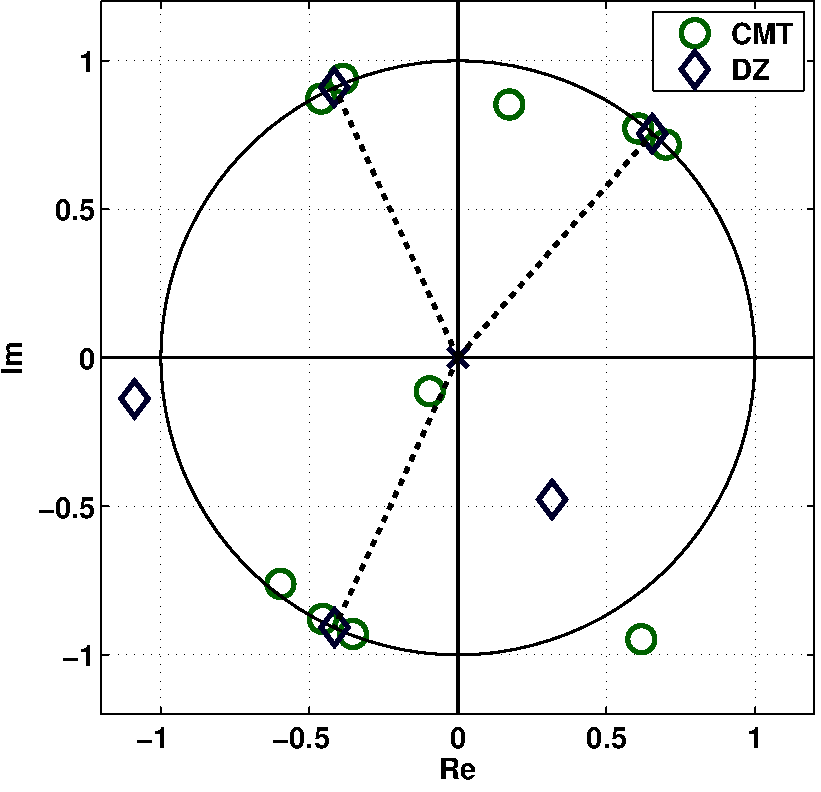
\includegraphics[width=3in]{./cmt_multi/cmt_pzplot_multi_D3.pdf}}
%   \subfloat[D = 4]{
%     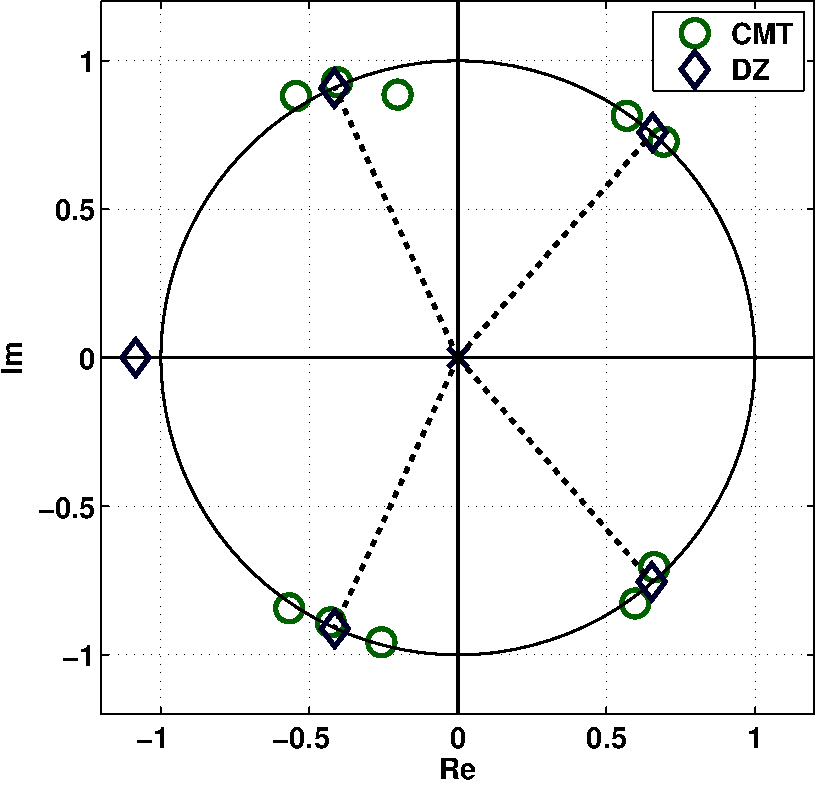
\includegraphics[width=3in]{./cmt_multi/cmt_pzplot_multi_D4.pdf}}
%   \caption{Zeros of CMT MVDR polynomial (green circles) and DZ MVDR
%     polynomial (black diamonds). The CMT MVDR ABF uses multiple zeros
%     at each interferer direction, depending on the chosen notch
%     width. The DZ MVDR ABF always uses two zero per interferer.}
% \label{fig:cmt-zeros-multi}
% \end{figure*}

% The
% DZ MVDR ABF consistently achieves lower output power under same
% conditions as observed in \figurename{}~\ref{fig:cmt-output-multi}.



% % Make clear that L snapshots are used to compute the weights first. Then we look at the output power over the same interval using the ECM for each instance.

% \subsection{Computational gain}
% \label{sec:computational-gain}
% \figurename{}\ref{fig:comp-gain} compares the computation time
% required by DZ MVDR (diamond markers) and SMI MVDR ABF (circle
% markers) implemented using ULAs with number of sensors ranging from
% $N = 11$ to $101$. The computation time for each ULA size was averaged
% over 3000 Monte Carlo experiments. Each experiment assumed $L = 2N$
% snapshots were available to implement the ABFs. DZ MVDR ABF clearly
% requires less computation time compared to the SMI MVDR ABF. The gain
% is more significant for longer arrays.

% % TODO: Consider including comp time for UC DZ MVDR to show that it
% % takes up more time than SMI MVDR.

% \begin{figure}[!t]
%   \centering
%   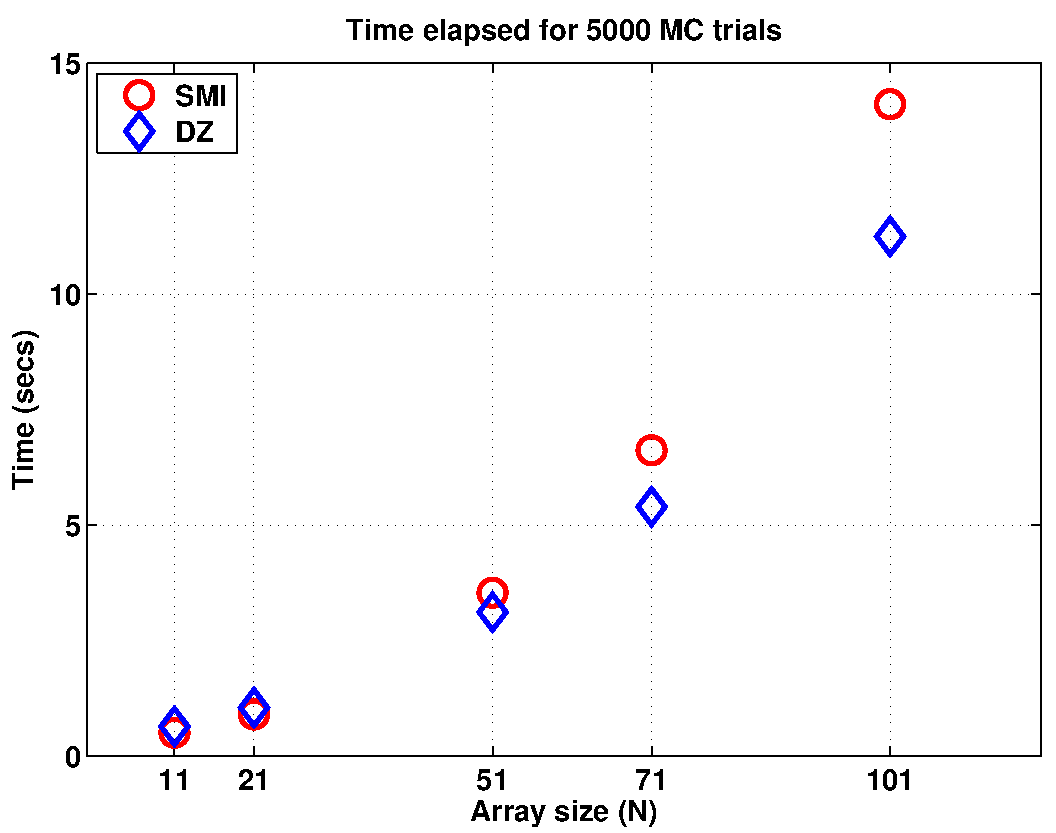
\includegraphics[width=2.5in]{comp_gain.pdf}
%   \caption{Computational gain using DZ MVDR over SMI MVDR.}
%   \label{fig:comp-gain}
% \end{figure}

%%% Local Variables:
%%% mode: latex
%%% TeX-master: "main"
%%% End:
